\noindent
Vì $f''(x) = 0$ khi $x = 0$ hoặc $2$, ta chia trục số thực thành các khoảng với các số này làm đầu mút và hoàn thành bảng sau.

\marginnote{%
  \centering
  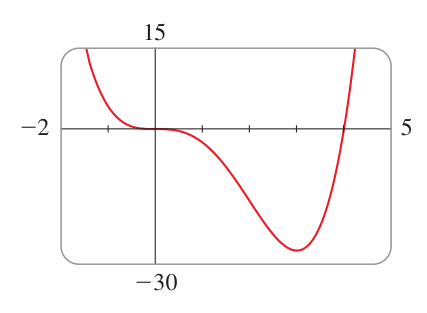
\includegraphics[width=\linewidth]{images/p0338_fig1.png}\\[4pt]
  {\small\textbf{\textsf{HÌNH 12}}}\\[2pt]
  {\small $y = x^4 - 4x^3$}
}[0pt]%
\begin{center}
\small
\renewcommand{\arraystretch}{1.3}
\setlength{\tabcolsep}{14pt}
\begin{tabular}{|c|c|c|}
\hline
\rowcolor{tableheader}
\textbf{Khoảng} & \boldmath$f''(x) = 12x(x - 2)$ & \textbf{Bề lõm} \\
\hline
$(-\infty, 0)$ & $+$ & hướng lên \\
$(0, 2)$        & $-$ & hướng xuống \\
$(2, \infty)$  & $+$ & hướng lên \\
\hline
\end{tabular}
\end{center}

\noindent
Điểm $(0, 0)$ là một điểm uốn vì đường cong chuyển từ lõm lên sang lõm xuống tại đó. Điểm $(2, -16)$ cũng là một điểm uốn vì đường cong chuyển từ lõm xuống sang lõm lên tại đó.\par
\noindent
Đồ thị của $y = x^4 - 4x^3$ trong Hình 12 củng cố các kết luận của chúng ta.\hfill\textcolor{stewartblue}{\rule{1.2ex}{1.2ex}}

\vspace{1em}
\noindent{\textcolor{stewartblue}{\rule{1.1ex}{1.1ex}}\quad \textbf{\large Phác thảo đồ thị}}\par\vspace{0.4em}
\noindent
Bây giờ chúng ta sử dụng thông tin thu được từ đạo hàm cấp một và cấp hai để phác thảo đồ thị của một hàm số.

\vspace{0.8em}
\noindent\textbf{\textcolor{stewartblue}{VÍ DỤ 7}}\quad Phác thảo đồ thị của hàm số $f(x) = x^{2/3}(6 - x)^{1/3}$.\par\vspace{0.4em}
\noindent\textbf{\textcolor{stewartblue}{LỜI GIẢI}}\quad Trước hết lưu ý rằng tập xác định của $f$ là $\mathbb{R}$. Việc tính hai đạo hàm đầu tiên cho ta

\marginnote{\raggedright\fontsize{8.5}{11}\selectfont Sử dụng các quy tắc tính đạo hàm để kiểm tra lại các phép tính này.}[-5pt]%
\[
f'(x) = \frac{4 - x}{x^{1/3}(6 - x)^{2/3}} \qquad\qquad\qquad f''(x) = \frac{-8}{x^{4/3}(6 - x)^{5/3}}
\]

\noindent
Vì $f'(x) = 0$ khi $x = 4$ và $f'(x)$ không tồn tại khi $x = 0$ hoặc $x = 6$, nên các số tới hạn là $0, 4$ và $6$.

\begin{center}
\small
\renewcommand{\arraystretch}{1.25}
\setlength{\tabcolsep}{8pt}
\begin{tabular}{|c|c|c|c|c|l|}
\hline
\rowcolor{tableheader}
\textbf{Khoảng} & \boldmath$4 - x$ & \boldmath$x^{1/3}$ & \boldmath$(6 - x)^{2/3}$ & \boldmath$f'(x)$ & \multicolumn{1}{c|}{\boldmath$f$} \\
\hline
$x < 0$     & $+$ & $-$ & $+$ & $-$ & nghịch biến trên $(-\infty, 0)$ \\
$0 < x < 4$ & $+$ & $+$ & $+$ & $+$ & đồng biến trên $(0, 4)$ \\
$4 < x < 6$ & $-$ & $+$ & $+$ & $-$ & nghịch biến trên $(4, 6)$ \\
$x > 6$     & $-$ & $+$ & $+$ & $-$ & nghịch biến trên $(6, \infty)$ \\
\hline
\end{tabular}
\end{center}

Để tìm các giá trị cực trị địa phương, ta sử dụng Kiểm định đạo hàm cấp một. Vì $f'$ đổi dấu từ âm sang dương tại $0$, nên $f(0) = 0$ là một cực tiểu địa phương. Vì $f'$ đổi dấu từ dương sang âm tại $4$, nên $f(4) = 2^{5/3}$ là một cực đại địa phương. Dấu của $f'$ không đổi tại $6$, do đó không có cực đại hay cực tiểu tại đây. (Có thể dùng Kiểm định đạo hàm cấp hai tại $4$ nhưng không dùng được tại $0$ hoặc $6$ vì $f''$ không tồn tại tại cả hai số này.)

Nhìn vào biểu thức của $f''(x)$ và nhận thấy rằng $x^{4/3} \geqslant 0$ với mọi $x$, ta có $f''(x) < 0$ với $x < 0$ và với $0 < x < 6$, còn $f''(x) > 0$ với $x > 6$. Do đó $f$ lõm xuống trên $(-\infty, 0)$ và $(0, 6)$ và lõm lên trên $(6, \infty)$, và điểm uốn duy nhất là $(6, 0)$. Sử dụng tất cả thông tin chúng ta đã thu thập được về $f$ từ đạo hàm cấp một và
